\section{Threshold Personalization Framework}
\label{sec:framework}

Fig.~\ref{fig:per-device-fpr} illustrates the operational consequence of heterogeneous
calibration: under B1 (client-averaged shared~$\tau$), per-device FPRs vary substantially
across the nine N-BaIoT clients, while B2 (per-client~$\tau$) reduces this dispersion for
the representative seed shown.
As an illustrative preview of the primary Regime~A pattern, Fig.~\ref{fig:per-device-fpr}
shows seed~0 only; inference uses the multi-seed results in Table~\ref{tab:regime_a}.

\begin{figure}[t]
  \centering
  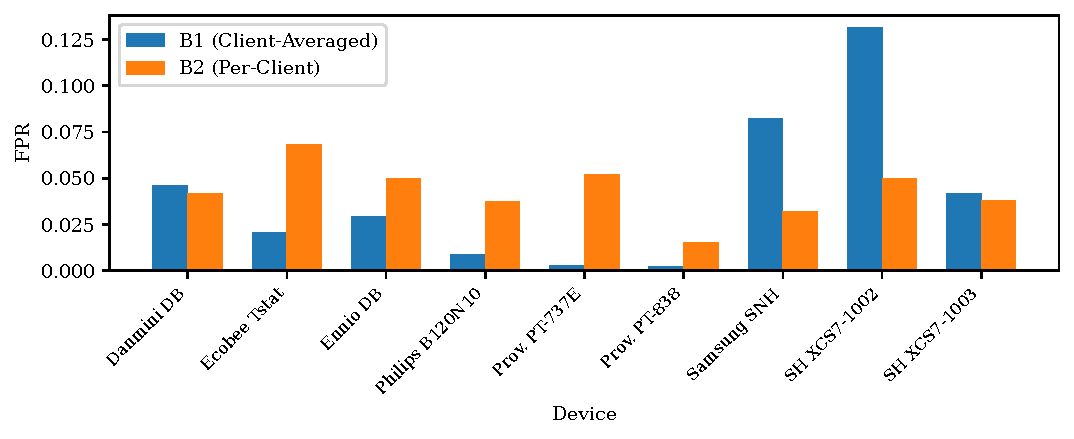
\includegraphics[width=\columnwidth]{figures/figure_1.pdf}
  \caption{Per-device FPR under B1 (Client-Averaged Shared~$\tau$) and B2 (Per-Client~$\tau$)
           for the nine N-BaIoT clients.
           \emph{Illustrative only (seed~0); multi-seed inference uses
           Table~\ref{tab:regime_a} and Table~\ref{tab:per_seed}.}}
  \label{fig:per-device-fpr}
\end{figure}

\begin{figure}[t]
  \centering
  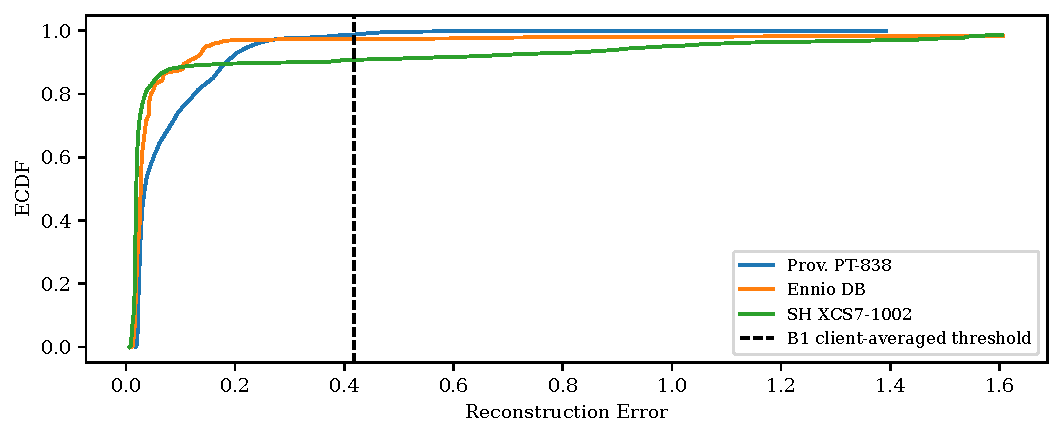
\includegraphics[width=\columnwidth]{figures/figure_2.pdf}
  \caption{Benign reconstruction-error empirical cumulative distributions for three
           representative N-BaIoT clients (seed~0).
           The shared threshold $\tau_{\text{global}}$ (B1, dashed) crosses each curve
           at a different exceedance fraction ($1 - F({\tau})$), producing unequal FPRs.
           Per-client thresholds (B2) set each client's $p_{95}$ independently,
           aligning benign-tail exceedance rates by construction.
           Attack distributions are not shown; they need not shift in parallel with benign tails,
           explaining the TPR/Macro-F1 tradeoff observed in Table~\ref{tab:regime_a}.}
  \label{fig:mechanism}
\end{figure}

\textbf{Pipeline.}
Each client holds benign traffic split into train, calibration, and test partitions;
attack data are reserved exclusively for evaluation and are never used to fit or tune thresholds.
A shared AE is trained with FedAvg via the Flower framework~\cite{beutel2020flower}
(identical training across B1--B4; B0 uses centralized pooling).
\emph{The AE is trained once per (dataset, regime, seed, $\alpha$) condition.}
After training, each client scores its calibration and test data under the fixed AE;
per-client score arrays are written to disk and reused by all threshold policies
without retraining.
Even when a run is budget-capped at 150 rounds, the same final AE state is shared
across all B1--B4 derivations, preserving the threshold-scope-only comparison.

\textbf{Threshold policies.}
Four policies operate on the shared score artifacts:
\begin{itemize}
  \item \textbf{B1 (Client-Averaged):}
        $\tau_{\text{global}} = \frac{1}{|\mathcal{K}_{\mathrm{elig}}|}\sum_{k\in\mathcal{K}_{\mathrm{elig}}} \tau_k^{(95)}$,
        applied uniformly to all clients.
        Pooled and weighted variants are sensitivity checks only
        (Table~\ref{tab:sensitivity_shared}).

  \item \textbf{B2 (Per-Client):} $\tau_k = \tau_k^{(95)}$ applied locally;
        zero additional uplink communication in a deployment where each client
        calibrates its threshold locally.

  \item \textbf{B3 (Family-Mean):} arithmetic mean of local thresholds within each device
        family (Regime~A only; requires a device taxonomy).

  \item \textbf{B4 (Cluster-Mean):} $k$-means on a 4-scalar fingerprint
        $[\mu_e, \sigma_e, \text{skew}_e, p_{95}(e)]$ (StandardScaler-normalized);
        $K{=}3$ for Regime~A, silhouette-selected for Regimes B/C.
        For silhouette selection (Regimes B/C), candidate $K \in \{2,3,4,5\}$;
        $k$-means uses \texttt{k-means++} initialization, $\texttt{n\_init}{=}10$,
        $\texttt{max\_iter}{=}300$, $\texttt{random\_state}{=}42$, applied after
        StandardScaler normalization of the fingerprint matrix.
        The four statistics are compact descriptors of the benign calibration-error
        distribution: $\mu_e$ captures location, $\sigma_e$ spread, $\text{skew}_e$
        tail asymmetry, and $p_{95}(e)$ the operating tail used by thresholding.
        They are distributional summaries for grouping, not privacy mechanisms.
        In Regime~A, $K{=}3$ is a practical fixed choice: with only 9 physical devices
        and coarse device-family structure, silhouette-based $K$ selection is unstable
        at small $n$; $K{=}3$ avoids overfitting cluster count to sampling noise.
        B4 requires sharing these distributional fingerprints, which carries nonzero
        metadata leakage risk (Section~\ref{sec:threats}).
\end{itemize}

Clients with fewer than $n_{\min}{=}100$ benign calibration samples are calibration-pending;
they receive $\tau_{\text{global}}$ as fallback and are excluded from CV(FPR).
\textbf{Evaluation.}
Each client evaluates FPR, TPR, balanced accuracy, and Macro-F1 on held-out test sets.
CV(FPR), CV(TPR), IQR(FPR), worst-client balanced accuracy, $P_{10}$ Macro-F1 (10th percentile
of per-client Macro-F1 across eligible clients), and coverage ratio are aggregated.
Seed-level deltas are summarized descriptively (mean, SD, range, sign consistency).
